% From repository root: pdflatex -output-directory=docs/figures docs/figures/diagrams/flow-diagram.tex
\documentclass{standalone}
\usepackage{tikz}
\usetikzlibrary{shapes, arrows, positioning, calc, arrows.meta, shadows, decorations.markings, backgrounds, fit}
\usepackage{amssymb}
\usepackage{amsmath}
\usepackage{pgfplots}
\pgfplotsset{compat=1.16}
\usepgfplotslibrary{patchplots}
\begin{document}
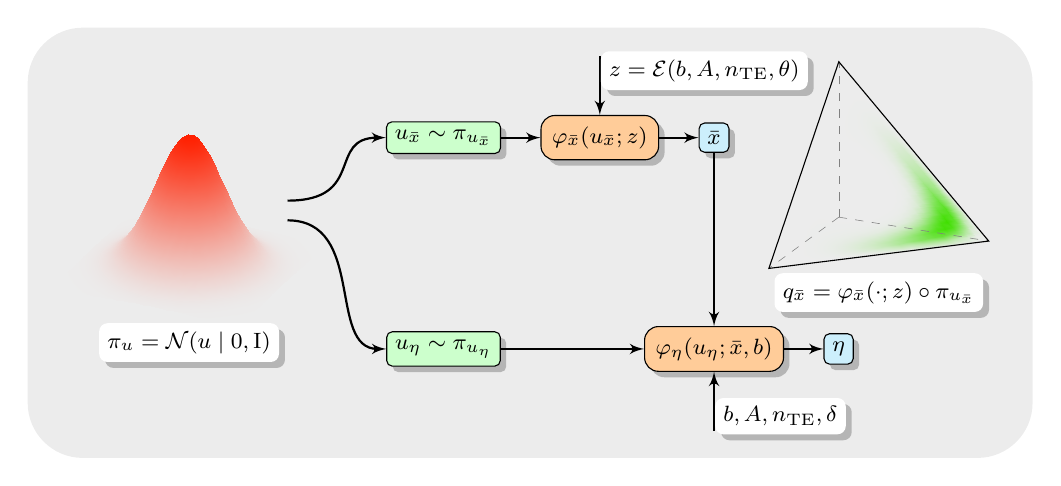
\begin{tikzpicture}[
        font=\footnotesize,
        flow_block/.style={rectangle, draw, fill=orange!40, align=center, rounded corners=5pt, drop shadow, inner sep=4pt},
        input_block/.style={rectangle, draw, fill=green!20, align=center, rounded corners=2pt, drop shadow, inner sep=3pt},
        output_block/.style={rectangle, draw, fill=cyan!20, align=center, rounded corners=2pt, drop shadow, inner sep=3pt},
        line/.style={draw, -latex', line width=0.8pt},
        textnode/.style={fill=white!5, inner sep=3pt, rounded corners=3pt, drop shadow},
    ]
    \begin{axis}[
            name=gauss_box,
            at={(0,0)},
            anchor=east,
            width=3.5cm,
            height=3.5cm,
            hide axis,
            colormap={whitered}{color(0cm)=(gray!15); color(1cm)=(red!75!orange)},
            domain=-3:3, y domain=-3:3,
            samples=50,
            scale only axis,
        ]
        \addplot3[surf, shader=interp] {exp(-x^2/2 - y^2/2)};
    \end{axis}
    \node[below=-0.2cm of gauss_box, align=center, textnode] (pi_node) {$\pi_u = \mathcal{N}(u \mid 0, \mathrm{I})$};
    \node[input_block, right=0.75cm of gauss_box.east, yshift=0.8cm] (u_x_node) {$u_{\bar{x}} \sim \pi_{u_{\bar{x}}}$};
    \path[line] ($(gauss_box.east)+(-0.5cm,0cm)$)
    .. controls ($(gauss_box.east)+(0.5cm,0cm)$) and ($(u_x_node.west)+(-0.75cm,0cm)$)
    .. (u_x_node.west);
    \node[flow_block, right=0.5cm of u_x_node] (flow_node) {$\varphi_{\bar{x}}(u_{\bar{x}}; z)$};
    \path [line] ($(flow_node.north)+(0,0.75cm)$) -- node[near start, right, textnode] {$z = \mathcal{E}(b, A, n_{\mathrm{TE}}, \theta)$} (flow_node.north);
    \path[line] (u_x_node.east) -- (flow_node.west);
    \node[output_block, right=0.5cm of flow_node] (x_node) {$\bar{x}$};
    \path [line] (flow_node.east) -- (x_node.west);
    \begin{axis}[
            name=simplex,
            at={($(x_node.east)+(0.5cm,-0.5cm)$)},
            anchor=west,
            width=3.0cm,
            height=3.0cm,
            view={115}{20},
            xmin=0, xmax=1, ymin=0, ymax=1, zmin=0, zmax=1,
            domain=0:1, y domain=0:1,
            samples=51,
            colormap={whitered}{color(0cm)=(gray!15); color(1cm)=(green!75!orange)},
            axis equal image,
            axis lines=none, ticks=none, hide axis,
            trim axis left, trim axis right,
            scale only axis,
            enlargelimits=false,
            clip mode=individual,
        ]
        \addplot3[
            surf,
            shader=interp,
            samples=30,
            point meta={x^2.5 * y^6 * z^2.5 * (1/3^3 - x * y * z)^5},
        ]
        ({x}, {(1 - x)*y}, {1 - x - (1 - x)*y});
        \draw[black!50, very thin, dashed] (axis cs:0,0,0) -- (axis cs:1,0,0);
        \draw[black!50, very thin, dashed] (axis cs:0,0,0) -- (axis cs:0,1,0);
        \draw[black!50, very thin, dashed] (axis cs:0,0,0) -- (axis cs:0,0,1);
        \draw[black] (axis cs:1,0,0) -- (axis cs:0,1,0) -- (axis cs:0,0,1) -- cycle;
    \end{axis}
    \node[below=-0.25cm of simplex, align=center, textnode] at (simplex.south) {$q_{\bar{x}} = \varphi_{\bar{x}}(\cdot; z) \circ \pi_{u_{\bar{x}}}$};
    \node[input_block, below=2.25cm of u_x_node] (u_n_node) {$u_{\eta} \sim \pi_{u_{\eta}}$};
    \path[line] ($(gauss_box.east)+(-0.5cm,-0.25cm)$)
    .. controls ($(gauss_box.east)+(0.5cm,-0.25cm)$) and ($(u_n_node.west)+(-0.75cm,0cm)$)
    .. (u_n_node.west);
    \node[flow_block, align=center] (laplace_node) at (x_node.south |- u_n_node.east)  {$\varphi_{\eta}(u_{\eta}; \bar{x}, b)$};
    \path [line] ($(laplace_node.south)+(0,-0.75cm)$) -- node[near start, right, textnode] {$b, A, n_{\mathrm{TE}}, \delta$} (laplace_node.south);
    \path [line] (x_node.south) -- (laplace_node.north);
    \path[line] (u_n_node.east) -- (laplace_node.west);
    \node[output_block, right=0.5cm of laplace_node] (log_s_node) {$\eta$};
    \path [line] (laplace_node.east) -- (log_s_node.west);
    \begin{scope}[on background layer]
        \node[fill=gray!15, rounded corners=0.7cm,
            fit={(current bounding box.south west) ($(current bounding box.north east)+(0.25cm,0cm)$)},
            inner sep=0.3cm] {};
    \end{scope}
\end{tikzpicture}
\end{document}
